\documentclass[a4paper]{article}
\usepackage{apacite}
\usepackage{xurl}
\usepackage{tabularx}
\usepackage{siunitx}
\usepackage{amsmath}
\usepackage{rotating}
\usepackage{colortbl}
\usepackage{multirow}
\usepackage{graphicx}
\usepackage{caption}

% No more than 3000 words.


\begin{document}


\begin{titlepage}
    \title{\textbf{How does the economy development (measured using GDP per capita) affect the CO2 emission per capita during 2002 - 2022? \\ \small ESS SL Internal Assesment}}
    \author{Zhou Changhui}
    \date{\today}
    \maketitle
    Environmental issue: Green house gas emission and global warming
    %\tableofcontents
\end{titlepage}

\section{Introduction and background knowledge}

Climate change is one of the most concerned issues in the modern world. Due to the rapid growth in population and industrialization, a steep increase in the emission of green house gases (GHGs) have occured and resulted in may serious problems. In addition to the most known threat, sea-level rising \cite{hansen2013climate}, scientists have found numerous other consequences including but not limited to affecting food security and human health \cite{co2foodhumanhealth}, increased risk of heavy metal contamination in soil \cite{co2heavymetal}, and harm to microbes and the ecosystem \cite{co2microbes}. Carbon dioxide is a side-product of grazing, fossil fuel combustion and other industrial practices, which is considered the most major GHG that is responsible for global warming, which requires urgent attention and action \cite{solomon2009irreversible}. 

Human socity has made many major progesses since then. Kyoto Protocal (1997) binded emission reduction targets for developed countries and marked the first time that global warming is globally recognized as a international issue. In Paris Agreement (2015), nearly all nations committed to “Nationally Determined Contributions” (NDCs) to reduce emissions, marking a full-scale recognision of the urgency of mitigating global warming. Many recent technology development and policies favoring green energy and decarbonization also played a major role in the reduction of GHG emission. However, many challenges are still present on the path to full solution of global warming. % Examples probably US not accepting, EU(DE) getting coal plants back, people arguing the amount of responsibility to take and balance between CO2 and development, etc. 

Economy development is another factor commonly considered when talking about GHG emissions, as GHG emissions are commonly considered a side effect of economy development. In this study, the economy development is measured using GDP per capita, which is a common indicator of economic development. GDP per capita provides a simple, standardized way to compare the average economic output per person across countries and has a strong corrlation with the material affluence of a nation \cite{UNDP_HDR_2023}.

\textbf{Research question: How does the economy development (measured using GDP per capita) affect the CO2 emission per capita?}

\section{Strategy (carbon budget)}

Humans have set multiple critical values to limit the global warming, the most famous one being the 1.5$^\circ C$ from the 2015 Paris Agreement. To achieve that, only a certain amount of green house gases can be released to the atmosphere. A \textit{carbon budget} is estimated the total amount of carbon dioxide (CO$_2$) that humanity can emit while still having a specified probability of keeping global warming under a certain threshold, calculated using the approximately linear relationship between the rise in golbal average temperature and the amount of CO$_2$ emitted \cite{esd-15-387-2024}. When such budget is calculated, countries can hold conferences and negotiations to allocate the budget, and divide them further inside the nations. If all countries follow the agreement and manage to control the carbon emission within the budget, the global warming can be kept under control.

This strategy provided a numerically quantifiable, methodologically viable solution to the problem of climate change, with some consideration of the different economical status of countries. It sets a clear boundary for each nation. Governments can therefore know how much they should invest in green technology research, and to what extent should they impose carbon taxes, with limited effect to the economy. 

However, there are still flaws of the action that prevents it from fully taking place. First, it is challenging to accurately estimate not only the budget, but also the ongoing GHG emission due to various sources \cite{essd-budget}. Unlike fossil fuels, the emission of GHGs due to deforestation, grazing and permafrost thawing is hard to be considered into the budget. Second, it is difficult for countries to reach an agreement on the budget. Developed countries may argue that they provided the most advanced green technology and pioneered in the climate acts, and should therefore be granted more carbon budgets, while developing countries may have an economy heavily dependent on fossil fuel and took up much less historical carbon budget, and demand for the right to emit more carbon dioxide. Third, right-wing politicians and some people may not think global warming is a real problem and do not want to take any action to reduce the emission. They do not want to sacrifice the lifestyle for some distant problem that does not even sound problematic to them. Finally, it is hard to monitor if one country is following the agreement or not, as there is no central authority that can enforce the budget without the consent of the countries. % Might need to add cites. 

\section{Hypothesis and reasoning}

\subsection{Cross-sectional Hypothesis}

Generally speaking, we divide a country's economy into three catogories: primary (agriculture), secondary (industry) and tertiary (service). Nowadays, not only is energy highly dependent on fossil fuel in most countries, but it also plays a pivotal role in most countrie's industry and production. This draws close connection between CO2 emission per capita and GDP per capita.

Primary sector-dominant economies are countries that did not undergo industrialization. They generally constitute of a large amount of farming, grazing and fishing. These economy practices are natural and require little fossil fuel. However, these industries also tend to be less productive, which would result in low GDP per capita. These countries tend to be low-income or developing countries at an early stage, like Afganistan, Chad, or some sub-Saharan countries.

Secondary sector-dominant economies are emerging or newly industrialized countries. They typically feature rapid industrial growth, especially in manufacturing and construction, and decline in agriculture. This transition from primary to secondary sector, however, requires a large amount of energy and chemical ingredients that comes from fossil fuel, which can significantly increase the CO2 emissions per capita. These economies are generally middle-income or developing countries, like China, India, or Brazil, with moderate GDP per capita.

Tertiary sector-dominant economies are generally developed countries, with mechanized mass production of agriculture and automated industry being the primary and secondary sections and service industry being the dominat tertiary section. With advanced technology and high productivity, these economies are generally high-income or developed countries, like the US, UK, or Japan, with high GDP per capita. Although these economies can produce GDP way more efficiently and the governments are generally more aware of the environmental issue, the CO2 emission per capita can still be high due to large number of devices consuming energy and expensive lifestyle.

Some countries may not fit perfectly into these catogories. The resource rich-countries like Qatar or Saudi Arabia have high GDP per capita but did not go through a typical industrialization path. Tourism-dependent countries can develop strong tertiary industry without a developed secondary section. So outliers of the three catogories are also possible.

By concluding the three catogories, we can see that GDP per capita and CO2 emission per capita are expected to be positively correlated nationwise. 

\subsection{Longitudinal Hypothesis} %might need to talk about global average

Despite having economical crisis and the Covid pandemic, the economy during the 2002 - 2022 period is generally developing, so we can naturally hypothesize that GDP per capita is expected to exhibit an increasing trend in all of the countries studied.

The CO2 emission per capita is expected to show different trends. During 2002 - 2022, developing countries like China and India are shifting from primary sector, which mostly involved natural growth and little CO2 emission, to energy-intensive, CO2-emitting secondary sector. This change in economical emphasis is expected to result in an increase in CO2 emission per capita. On the contrary, developed countries like the US and the UK are shifting to the tertiary sector and their CO2 emission per capita is expected to be higher but decreasing. LDCs are expected to remain low in CO2 emission.

In fact, the Kuznet curve is commonly used to describe some side-effect of the economy increase which is expected to be limited by further growth, like inequality (as is used in Kuznet's origional studies) and GHG emission (as is used in this study). Kuznet curve hypothesizes an inverted U-shape curve on the emission-GDP graph. This means that the CO2 emission per capita is expected to be strongly correlated with GDP per at the early stage of development, but becomes less relevant and even negatively correlated in the later stage.

\section{Methodology}

This study requires large dataset around the world that can not be reproduced in laboratory conditions or revealed through survery, so secondary data is adopted to carry out the research.

This study uses secondary data obtained from \texttt{ourworldindata.org}. The dataset is publicly available and anonymized, ensuring no personally identifiable information is included. Data were used in compliance with the source's terms of use and citation requirements. No modifications were made to the original data. Therefore, no additional safety and ethical precautions are required.

Ourworldindata is generally considered a reliable source and both the variables can be calculated by commonly researched topics. The ultimate data sources are Global Carbon Budget (2024) and Bolt and van Zanden - Maddison Project Database 2023. Both are reliable enough to be used in this study.


\section{Results and analysis}

\subsection{Cross-sectional results}

The cross-sectional analysis is done by the scatter plot and linear-fit, as is shown in Figure \ref{fig.horizontal}. Data from 2002, 2012 and 2022 are chosen for analysis. Each country is represented by a dot, whose size is proportional to its total population in the graph. Some typical countries are highlighted in the graph.

\begin{figure}[ht!]
    \centering
    \caption{Scatter plot of GDP per capita and CO2 emission per capita.}
    \label{fig.horizontal}
    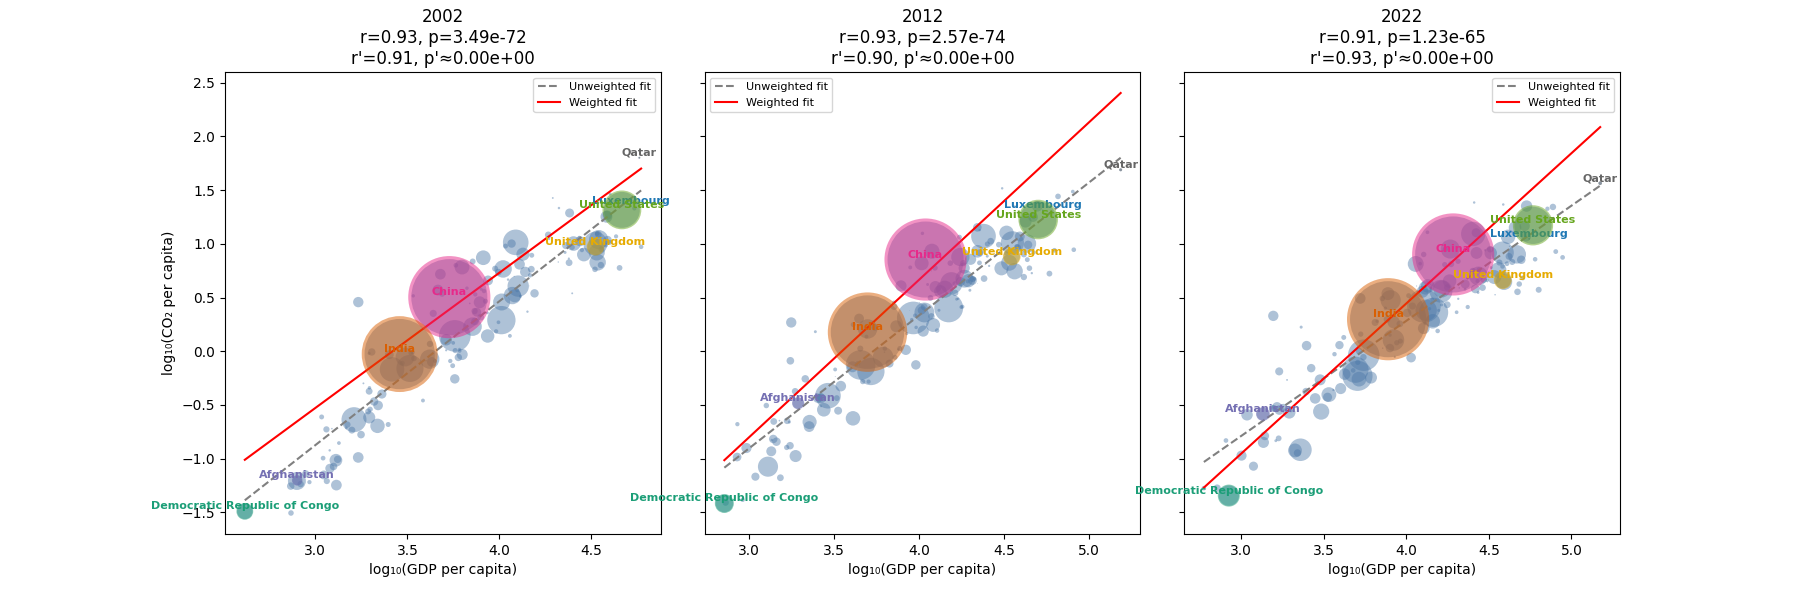
\includegraphics[width = \textwidth]{data/horizontal.png}
\end{figure}

Figure \ref{fig.horizontal} shows very strong correlation between the two variables. It can be noticed that almost every country is displayed close to the linear fit line, proving the strong correlation. Statistical tests support the trend, as a Pearson correlation coefficient of $r = 0.93 (2002), 0.93 (2012), 0.91 (2022)$ is calculated for unweighted data and $r' = 0.91 (2002), 0.90 (2012), 0.93 (2022)$ for weighted data. All the coefficients are significantly higher than the common $0.75$ for a strong correlation in social sciences. Additionally, the $p$ test for each set of data is less than $10^{-64}$, indicating that the correlation is statistically significant.

We can also notice that the pattern of the scatter plot, especially the relative position of the typical countries chosen, does not change much over years. Afganistan and D.R. Congo are the examples of war-torn, foreign-exploited third-world countries, displayed in the left-bottom of the graph. China and India are the examples of large developing economies, occupying the center of the graph. The US, the UK and Luxembourg epitomizes developed nations at the right top of the graph, while Qatar, as the resource-rich fossil fuel exporter, being the outlier at the very right top corner. 

However, some transition can also be noticed in the graph. There used to be a clear boundary between the developing and the developed world in the left figure, but the gap is getting smaller and less significant as the countries in the center are moving up-right as they get industrialized, probably because of technology development and globalization. China and India both occupied a righter and upper position in 2022 compared to 2002, due to the industrialization and structural economy change to secondary industry. Unlike most other countries, the UK showed a decline in CO2 per capita during the process, largely thanks to the policies in favour of decoupling CO2 from economy development. The energy generation, manufacturing, water supply, and transport played vital roles during the process \cite{noco2gdpuk}. However, some of the reduction is dependent on offshoring energy-intensive manufacturing to developing countries \cite{peters2011growth}. 

\subsection{Longitudinal results} % might need pearson, delta pearson and so on

The longitudinal analysis is done by plotting GDP per capita, CO2 emission per capita and their ratio over time, as is shown in Figure \ref{fig.vertical}.

\begin{figure}[ht!]
    \centering
    \caption{Variables' change over time}
    \label{fig.vertical}
    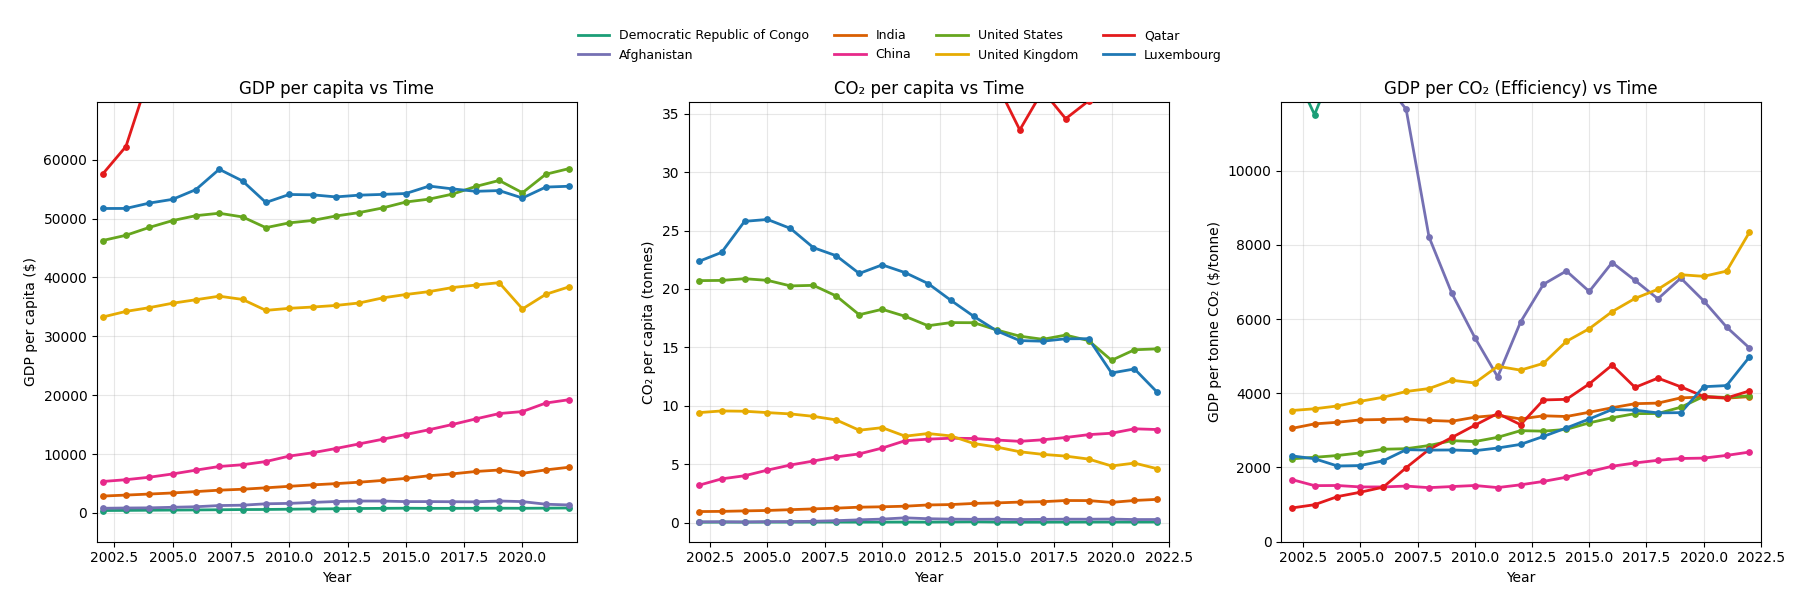
\includegraphics[width = \textwidth]{data/vertical(rescale).png}
\end{figure}

Figure \ref{fig.vertical} shows various information about the trend of the two variables. Most countries showed constant growth throughout the period except for 2008 (2008 finantial crisis) and 2020 (Covid-19 pandemic) which resulted in an abrupt downturn. This supports our prediction on GDP per capita. There is a significant gap between the developing and developed countries chosen in the graph. Despite all growing, the US, China and India showed a quicker increase in GDP per capita as the US benefited greatly from the globalization and China and India industrialized rapidly. Qatar's oil industry grew so rapidly that it was one of the country that had the highest GDP per capita and increase in GDP per capita during the period. D.R. Congo and Afganistan remains poor due to lack of source for economical growth.

As is hypothesized, developed countries, namely the US, the UK and Luxembourg transitioning from secondary economy to tertiary economy decreased their CO2 emission per capita thanks to technology development, policy reformation and relocation of the secondary industry to developing areas. Developing countries, especially China which just get industrialized, showed very rapid growth in CO2 emission per capita, even exceeding some developed countries like the UK. Qatar's oil industry remains to contribute to the highest CO2 emission per capita, while D.R. Congo and Afganistan remains low in CO2 emission due to lack of industry.

We can also notice that the GDP made from each tonne of CO2 is also increasing over time. This may attribute to the development of green technology and the prosperous tertiary econonomy that does not produce as much green house gases. Such growth is more prominant in developed countries as they tend to have more advanced technology and more efficient production.

As we can conclude from these trends, the CO2 emission can be the side effect of one source of GDP growth (as in manufacturing and energy generation), but the developed countries have already been decoupling CO2 emission from GDP growth, which yeild some fruitful results. This possibilty of decoupling CO2 from GDP growth showed that the CO2 emission per capita is not a necessary indicator of GDP per capita and there positive correlation, though prevelant in the global scale, can be mitigated using technology and active policy making. % supporting materials needed

\section{Conclusion}

To conclude, the research on data showed clear trends and successful statistic tests supporting the initial hypothesis. The cross-sectional analysis studied the similarity and differences across nations and revealed the strong correlation between CO2 emission per capita and GDP per capita. Such correlation testified the role of fossil fuel in the past economical development that shaped the international society nowadays. On the other hand the longitudinal analysis partially strengthened the correlation between the two variables with data from developing countries but also highlighted the decoupling of these two factors and predicted future less significant or negative correlation between the two variables. The outcome fits with the Kuznet model and indicated that most of the countries are still climbing the "peak" of the Kuznet curve in the past decades.

\section{Evaluation}

\begin{itemize}
    \item \textbf{Limited time range:} 2002 - 2022 was selected because of data availability and simplicity of analysis, as some data prior to 2002, especially the one of LDCs are not available for analysis. This can result in some historical factors and trends being not included in the analysis. It would be better if more data is available. Some analysis on the limited areas where data is available can be conducted as well.
    \item \textbf{Log-log scale:} Log-log scale is used because the exceptional high value of some developed countries make developing countries squeeze together in the graph. Subsequently, the linear-fit is conducted on the log-log scale to avoid distortions near the origion. Despite showing strong connection between the two variables, it does not necessarily show \textit{linear} correlation as the best fit line is not a straight line but a curve on the linear axis. Additional study on the linear scale can be conducted to compensate the flaw.
    \item \textbf{Nationwise data:} Data is collected country by country. This method can result in small countries such as Luxembourg having equal effect in data as the large countries such as the US, negelecting the large countrie's significance in CO2 emission and economy. This flaw is fixed by additional study on the data weighted according to the population. However, both studies focus on the cross-country comparisons while overlooking the intra-country differences. This can underestimate the regional and finantial impact of CO2 emission within one country, especially large countries like the US or China. This could be improved if more detailed data is available.
    \item \textbf{GDP per capita:} GDP per capita fails to consider or can underestimate factors like equality, non-market work, social well-being and technology development of a country. These are also significant factors that can affect the overall development and CO2 emission per capita. To put those factors into consideration, additional study on other factors like HDI (Human development index), GNI (Gross national income), GII (Global innovation index), etc. can be conducted.
\end{itemize}


\bibliographystyle{apacite}
\bibliography{cit.bib}

\end{document}